\documentclass{article}
\usepackage[T1]{fontenc}
\usepackage{lmodern}
\usepackage{graphicx}
\usepackage{amsmath,amssymb}
\usepackage[a4paper,margin=2cm]{geometry}
\usepackage[absolute,overlay]{textpos}
\setlength{\TPHorizModule}{1mm}
\setlength{\TPVertModule}{1mm}
\usepackage[indonesian]{babel}
\usepackage{hyperref}
\setlength{\emergencystretch}{2em}
% unit: Halaman 27

\begin{document}

% === Halaman 27 (python/native) ===

27

(a) Skema enkripsi mode CBC

(b) Skema dekripsi mode CBC

% deskripsi: gambar native xref 126
\noindent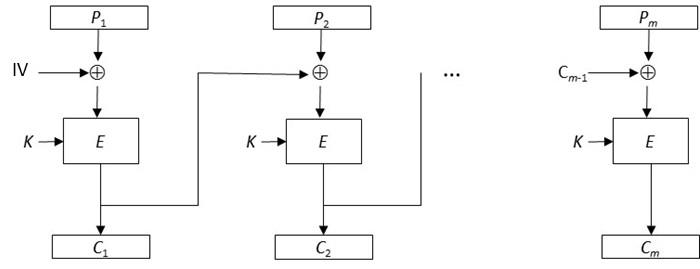
\includegraphics[width=0.85\textwidth]{../../images/python/page_027_img_01.jpeg}

% deskripsi: gambar native xref 127
\noindent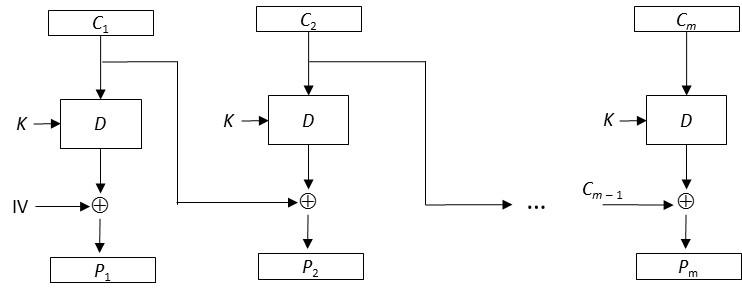
\includegraphics[width=0.85\textwidth]{../../images/python/page_027_img_02.jpeg}

% deskripsi: gambar native xref 128
\noindent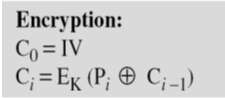
\includegraphics[width=0.85\textwidth]{../../images/python/page_027_img_03.png}

% deskripsi: gambar native xref 129
\noindent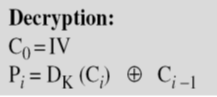
\includegraphics[width=0.85\textwidth]{../../images/python/page_027_img_04.png}

\end{document}
